\chapter{结合图路径和局部邻域的Transformer模型}

本章主要对结合图路径和局部邻域的Transformer模型TKGE-PN的总体设计和模块的具体实现进行了介绍。主要包括对基于图神经网络的方法以及NATLP模型存在问题的分析、模型的总体框架设计、基于有偏随机游走的图路径采样算法的设计、Path-Transformer路径编码模块以及Neighbor-Transformer局部领域编码模块的具体设计。

\section{现有问题分析}
NATLP模型对传统的Transformer模型的自注意力机制的计算方式进行改进,捕获了中心实体局部邻域内的结构信息,将Transformer模型应用到了知识图谱补全中,解决了先前基于图神经网络的方法模型表达能力差、对邻居实体之间相互依赖学习不足的问题。

但是,NATLP模型依然存在缺陷,由于依然基于中心实体的局部邻域进行推理,NATLP并没有解决基于图神经网络的知识图谱嵌入方法对于于长距离依赖学习不足的缺点。在知识图谱中,长距离的含义是实体间通过边连接需要经过多个中间节点。长距离依赖反映出实体之间较为间接的联系,这种联系在理解实体间复杂关系的层面上是非常重要的。例如,某一个历史人物与某一个现代组织之间可能存在长距离依赖,尽管他们之间直接的联系很少,但通过一系列历史事件和影响,可以构建出两者之间的联系,因此捕捉长距离依赖有益于推理和查询知识图谱的高阶模式。

基于图神经网络的方法主要是通过利用中心实体的局部邻域中蕴含的信息来完成知识图谱的补全。每层图神经网络只能学习到中心实体的一跳邻居的信息,这导致模型能够很好的捕捉知识图谱中的短距离依赖,而对于实体和实体之间的长距离依赖的学习不够充分。虽然其可以通过堆叠多层图神经网络让中心实体感知到距离更远的其他实体,但这样的方式只在层数较低(例如一到两层)时有效,之后随着层数的进一步增加,模型的性能反而会出现快速的下降,这主要是由过平滑问题(over-smoothing)导致的,即因为感受野的重叠而导致不同节点的表示过于相似无法进行区分。文献\cite{over-smoothing}对这种现象进行了系统和定量的研究,通过引入定量指标,发现导致过平滑的关键因素是节点接收到的有效信息与噪声比例过低,结果如图\ref{information-noise}所示,该图来自于文献\cite{over-smoothing}原文。在每层神经网络中,节点都会聚合其所有邻居节点的信息并传递给下一层,这导致模型引入了大量的噪声信息。因此基于图神经网络的方法一般只能捕捉单个实体附近1-2跳内的局部信息,而缺乏利用长距离乃至全局信息的能力。
\begin{figure}[htb]
  \centerline{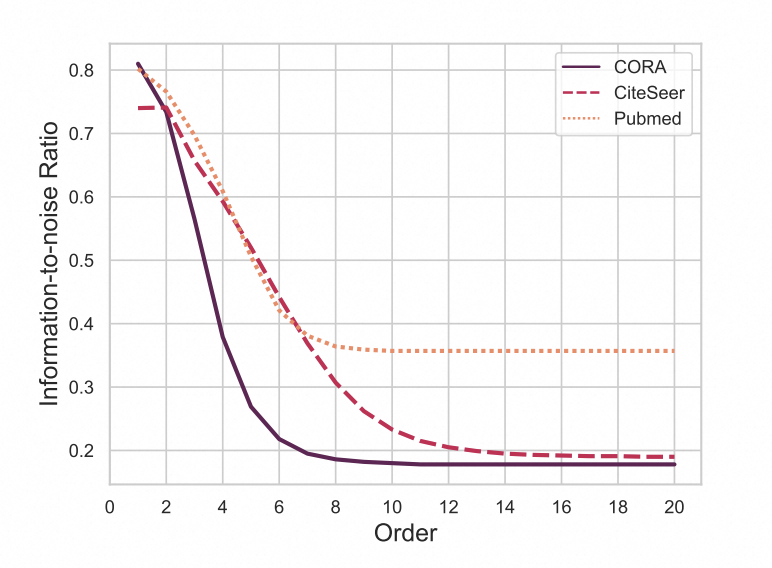
\includegraphics[width=0.7\textwidth]{pic/information-noise.png}}
  \caption{网络层数对信噪比的影响}
  \label{information-noise}
\end{figure}

为了解决以上问题,本文提出了一种基于Transformer的结合图路径和局部邻域的知识图谱嵌入方法(A Transformer-based Knowledge Graph Embedding Model Combining Graph Paths and Local Neighborhood,TKGE-PN)。基于图神经网络的方法的成功证明了实体的局部邻域蕴含了丰富的信息,但知识图谱的结构信息除了图神经网络使用的局部邻域之外还有多种表达形式,例如图路径以及子图。在知识图谱中,图路径被定义为图谱中的实体-关系链,由不同三元组收尾相连组成,例如(Yao Ming, Born In, Shanghai, City Of, China)。相对于局部邻域,图路径能够帮助模型更好地捕获实体和实体之间长距离的依赖,如图\ref{long-term-dependency}所示。结合图路径和邻域信息,模型能够更好地学习长短距离依赖的同时避免过度平滑问题的出现。同样的,和NATLP类似,和GNN浅层的神经网络结构相比,Transformer的自注意力机制能够给模型带来更强大的表达能力。本文提出的TKGE-PN以中心实体作为起点,采用有偏随机游走算法对图路径进行采样,并通过基于Transformer的图路径编码模块和邻域信息编码模块对图谱中的长距离和短距离结构信息进行编码。此外本文为图路径编码模块设计了一个掩蔽实体关系预测任务,以确保模型能够充分学习图路径之间的长距离依赖。

\begin{figure}[htb]
    \centerline{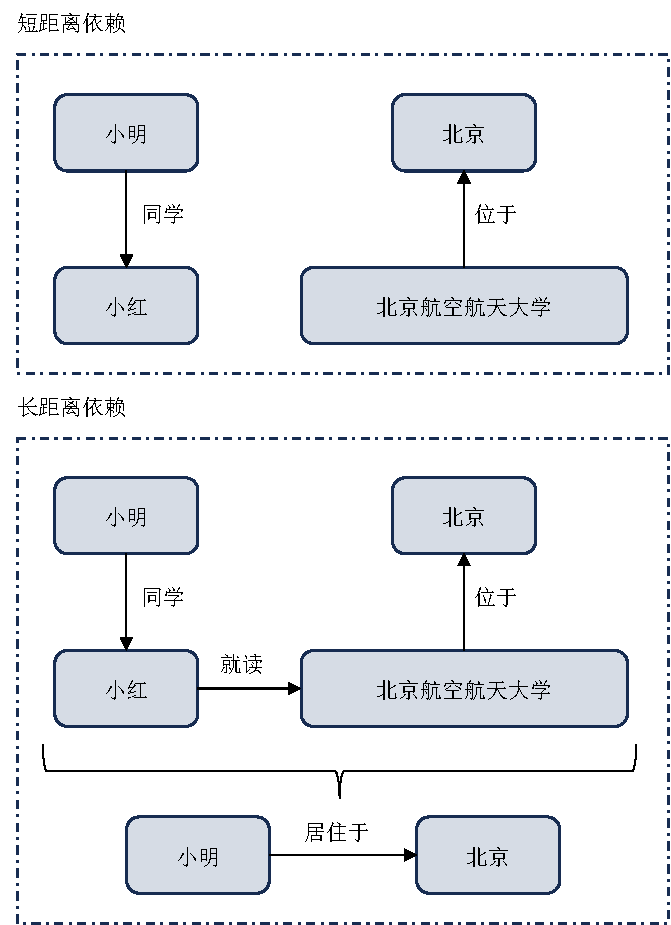
\includegraphics[width=0.5\textwidth]{pic/long-term-dependency.pdf}}
    \caption{知识图谱中的短距离距离信息和长距离信息}
    \label{long-term-dependency}
  \end{figure}

\section{TKGE-PN模型设计}

\subsection{符号定义}
为了方便说明论文提出的TKGE-PN模型的实现细节,本节对TKGE-PN模型中的关键概念和相关的数学符号进行了定义,具体内容参见表\ref{definition_TKGE-PN}。

\setlength{\tabcolsep}{20pt}

\renewcommand\arraystretch{1.2}
\begin{longtable}[htbp]{cc}
  % 首页表头
  \caption{TKGE-PN模型中的符号定义}
  \label{definition_TKGE-PN}\\
  \toprule
  符号  & 说明\\
  \midrule
  \endfirsthead
  % 续页表头
  \caption{TKGE-PN模型中的符号定义}\\
  \toprule
  符号  & 说明 \\
  \midrule
  \endhead
  % 首页表尾
  \hline
  % \multicolumn{2}{r}{\small 续下页}
  \endfoot
  % 续页表尾
  \bottomrule
  \endlastfoot
  
  $\mathcal{G}$   &   知识图谱      \\
  $\mathcal{E}, \mathcal{R}, \mathcal{T}$   &   实体集合、关系集合、边集合      \\
  $\mathcal{G}^\prime$  &  拓展后的知识图谱      \\
  $\mathcal{R}^{\prime}$   &   拓展后的关系集合      \\
  $\mathcal{T}^{-1}$   &   逆关系边集合      \\
  $\mathcal{T}^{\prime}$   &   拓展后的边集合      \\
  $(s,r,?)$  &   待遇测的三元组      \\
  $s$   &   头实体即中心实体      \\
  $o$   &   尾实体即目标实体      \\
  $e$   &   实体      \\
  $r$   &   关系      \\
  $r^{-1}$   &   关系$r$的逆关系      \\
  $\boldsymbol{s},\boldsymbol{o}$ & 头实体嵌入和尾实体嵌入\\
  $\boldsymbol{e},\boldsymbol{r}$ & 实体嵌入和关系嵌入\\
  $d$ &嵌入维度\\
  $\phi_{chk}$ & 棋盘式特征重组\\
  $\circledast$ & 循环卷积操作\\
  $f(\cdot )$ & ReLU激活函数\\
  $vec(\cdot)$ & 二维张量转化为一维向量\\
  $\omega_r$ & 特定于关系$r$的卷积层参数\\
  $\mathbf{W}_r$ &特定于关系$r$的全连接层参数\\
  $\boldsymbol{e}_{cls}$ & 特殊嵌入Class Token\\
  $\mathbf{TE}$ & 类型嵌入\\
  $a_{ij}$ & 第i个输入和第j个输入之间的注意力得分\\
  $dis(e_i,e_j)$ & 实体$e_i$与实体$e_j$之间最短路径的距离\\
  $deg(e)$ & 实体$e$的节点度数\\
  $\boldsymbol{o}_t$ & 模型预测的候选实体的嵌入\\
  $\sigma $ & sigmoid激活函数\\
  $p$ & 三元组正确概率\\
  $L$ & 模型损失\\
  $t_i$ & 第i个三元组的标签\\

\end{longtable}

和NATLP中的处理方式类似,为了确保信息的双向流动,TKGE-PN会对知识图谱进行拓展,为知识图谱中的每个事实三元组$(s,r,o)$添加对应的逆关系和逆三元组:

\begin{gather}
    \mathcal{R}^{\prime}=\mathcal{R}\cup\{ r^{-1} | r\in \mathcal{R}\}\\
    \mathcal{T}^{-1}= \{ (o,r^{-1},s)| (s,r,o)\in \mathcal{T}\}\\
    \mathcal{T}^{\prime} = \mathcal{T}\cup\mathcal{T}^{-1}\\
    \mathcal{G}^\prime = (\mathcal{E}, \mathcal{R}^\prime, \mathcal{T}^\prime)
\end{gather}

\subsection{模型总体结构}

本节主要对提出的基于Transformer的结合图路径和局部邻域的知识图谱嵌入方法TKGE-PN的总体结构进行介绍。和NATLP不同的是,TKGE-PN并没有采用编码器-解码器架构,而是利用Transformer自身的强大表达能力直接对目标实体的嵌入进行预测,这样的方式的优点是模型的性能不会受限于用作解码器的基于图神经网络的知识图谱嵌入方法的限制。

TKGE-PN模型主要由三个部分组成,首先是基于有偏随机游走的图路径采样算法,以中心实体为起点在图谱中采样多条图路径;随后Path-Transformer路径编码模块负责学习图路径中蕴含的长距离的语义信息并转换为向量表示;Neighbor-Transformer局部邻域编码模块接收来自Path-Transformer的输入,整合待遇测事实三元组以及多条图路径所构成上下文邻域信息并预测三元组得分。模型架构如图\ref{TKGE-PN_architecture}所示。

\begin{figure}[htb]
  \centerline{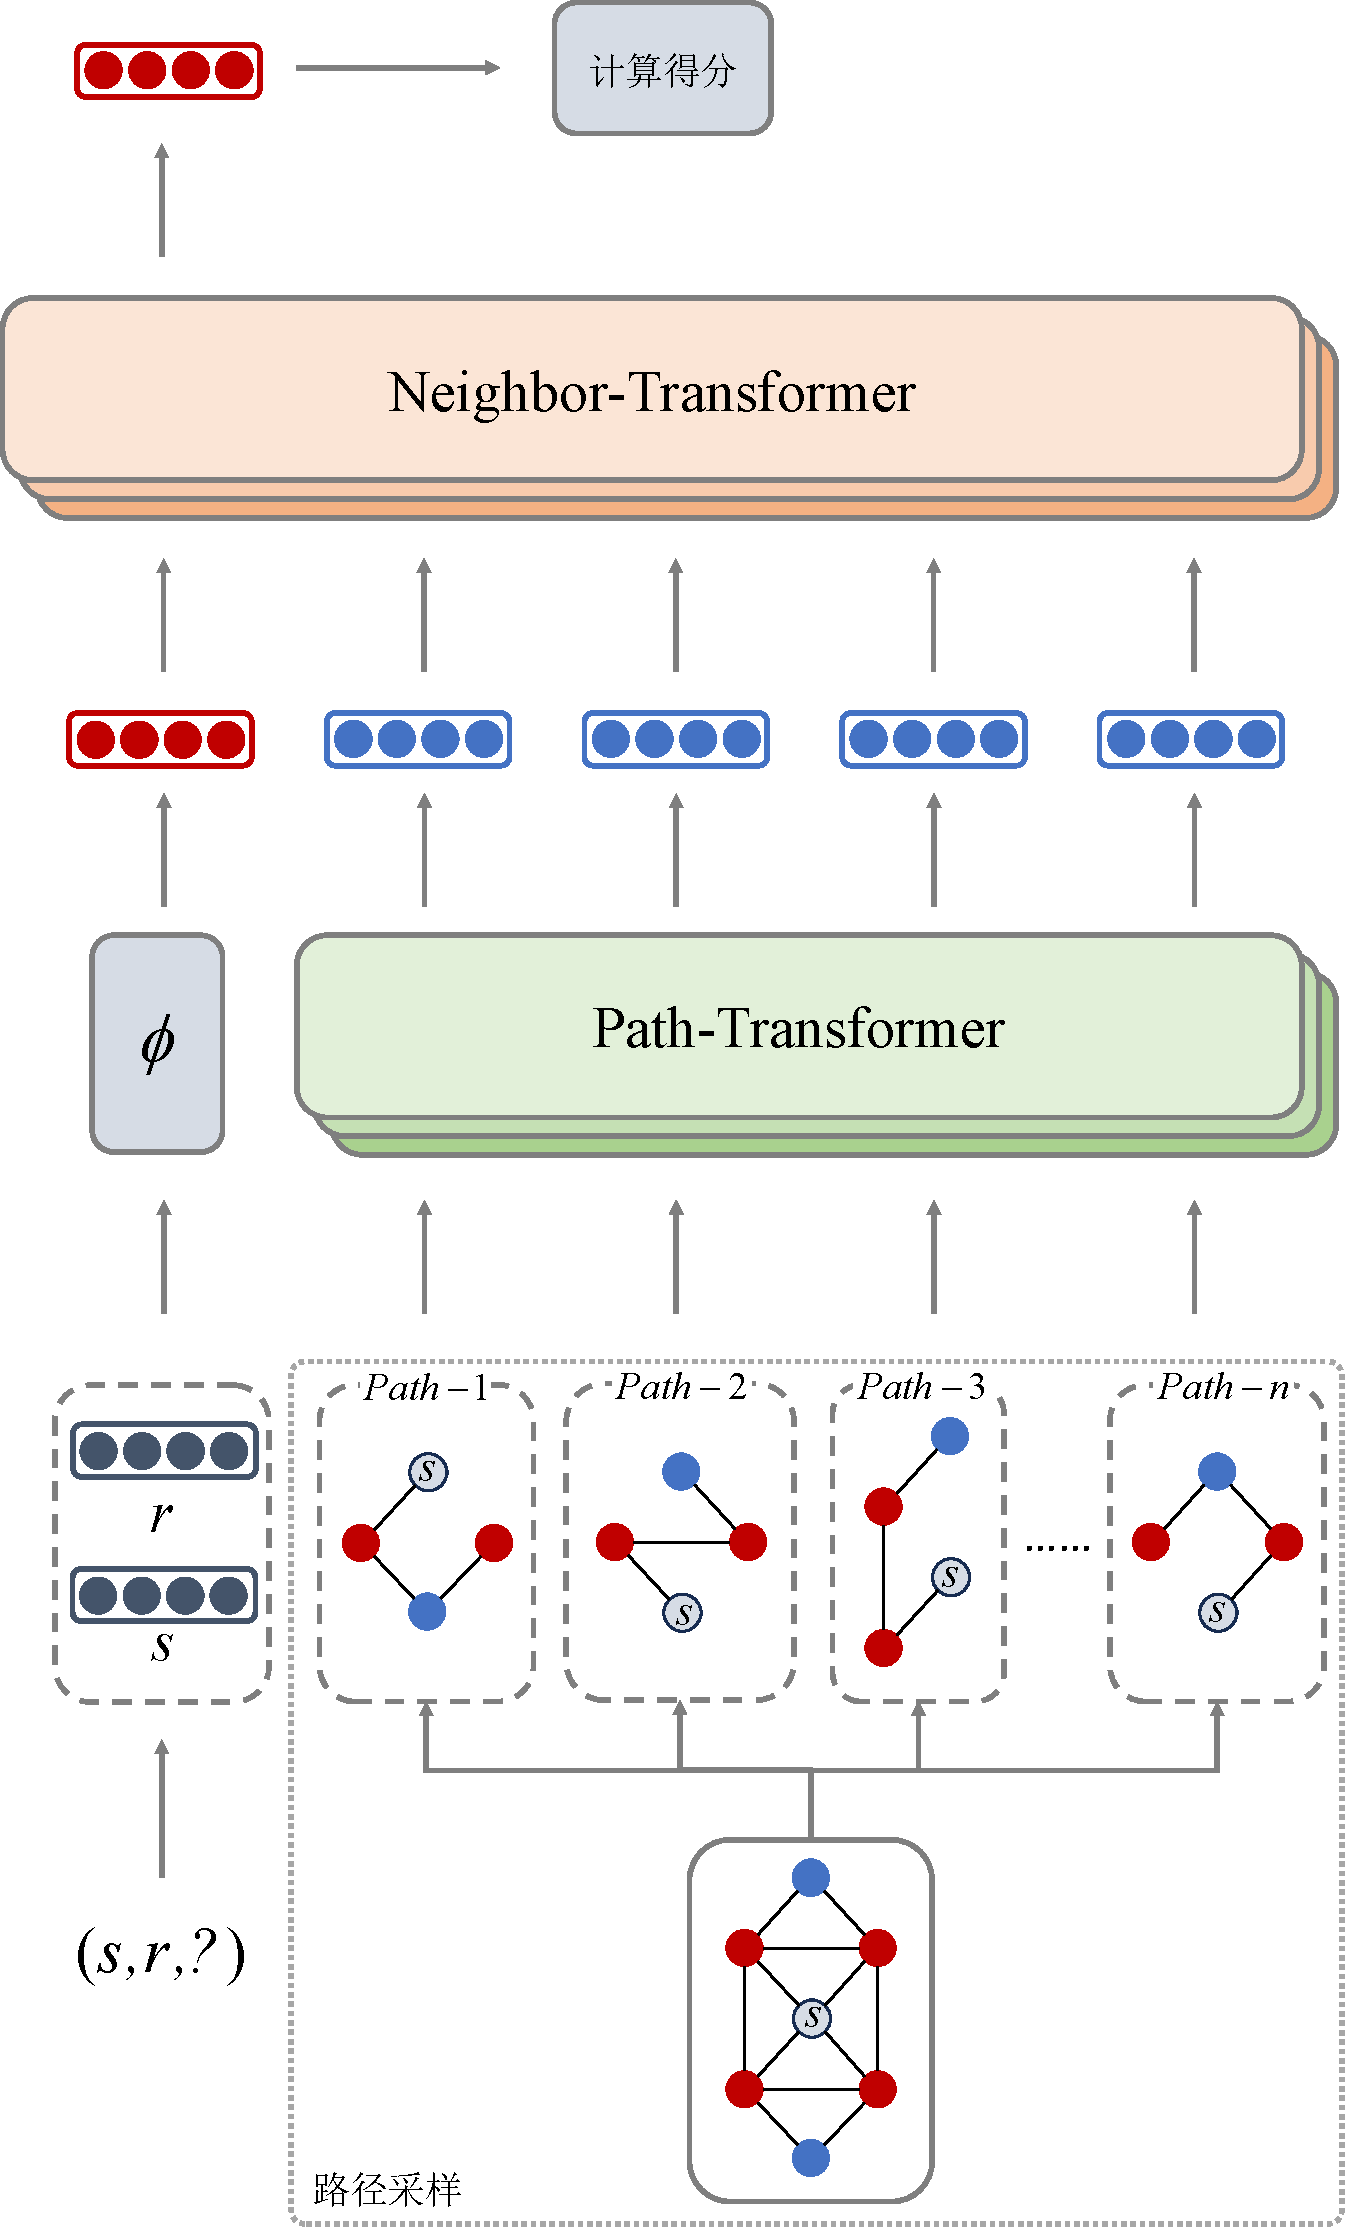
\includegraphics[width=1\textwidth]{pic/TKGE-PN_architecture.pdf}}
  \caption{TKGE-PN模型整体架构}
  \label{TKGE-PN_architecture}
\end{figure}
